\documentclass[11pt]{article}

\usepackage{amsmath}
\usepackage{amssymb}
\usepackage{enumitem}
\usepackage[final]{graphicx}
\graphicspath{{./project_structure.pdf}}

\author{Erik Sturzenhecker, Felix Thiele}
\title{A Start to the formalization of Linear Algebra in ForTheL}

\date{\today}

\begin{document}
\maketitle

\newpage 
\setcounter{tocdepth}{10}
\tableofcontents


\newpage 
\section{Introduction}
\subsection{Naproche}
In this project we build a linear algebra library in ForTheL with Naproche. ForTheL, which stands for Formal Theory Language, is a language that comes close to human language. This reduces many of the initial hurdles people encounter in the formalization of mathematics. Naproche can not only interpret ForTheL code, but is also backed with a strong Automated Theorem Prover, to which we shall refer to as e-prover. This makes many Proofs in our library easier, since some trivial steps can be skipped. At the same time this comes with massive performance issues, since checking this small library is a comparably very time intensive task.

\subsection{Results}
Some of the results given in this library are:
\newline
The \textbf{definitions} of:
\setlist{nolistsep}
\begin{enumerate}[noitemsep]
\item Groups, Rings, Fields
\item Vector spaces, Subspaces, Dual spaces
\item Homomorphisms, Endomorphisms, Automorphisms of vector spaces
\item Lists, Linear independence
\end{enumerate}
And the \textbf{proofs} of:
\setlist{nolistsep}
\begin{enumerate}[noitemsep]
\item A field is a vector space over itself.
\item The linear maps between $K$-vector spaces $V§$ and $W$ form a vector space Hom($K$,$V$,$W$).
\item If $f$ is linear, Ker($f$) is a subspace.
\item If $f$ is linear and Ker($f$) $=$ \{0\}, then $f$ is injective.
\item The endomorphisms of a $K$-vector space $V$ form a ring End($K$,$V$).
\item The invertible elements of a ring form a multiplicative group.
\item Any $K$-vector space $V$ can be embedded into the double dual space $(V^{*})^{*}$
\end{enumerate}

\newpage

\section{Formalization}
\subsection{Project structure}
Giving the project a treelike structure with a file to each topic ensures increased readability and scalability. 
In contrast to having one large file building up mathematics, this enables us to pick what files need to be imported to each file. 
Our structure is depicted in the graph below.

\begin{figure}[h]
\begin{center}
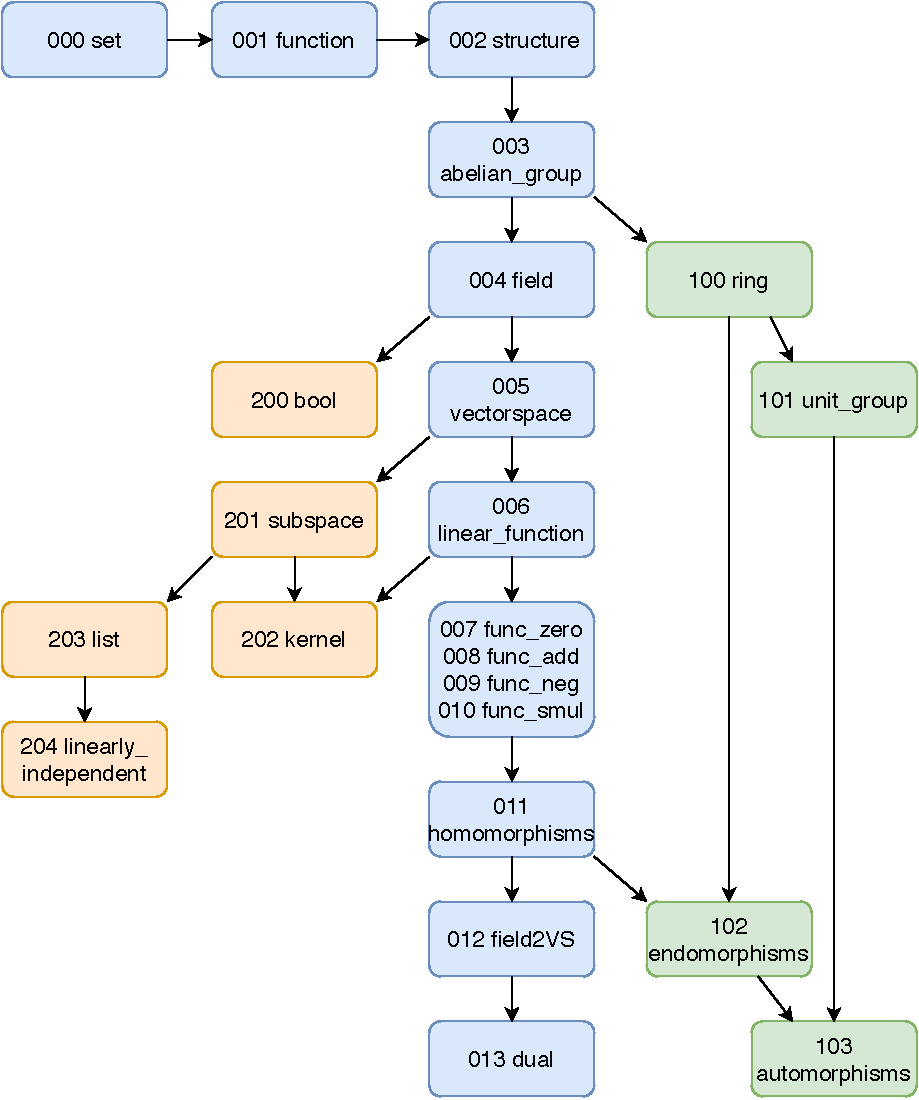
\includegraphics[scale=0.75]{./project_structure.pdf}
\end{center}
\end{figure}

\newpage

The e-prover is not fast enough to compile the entire library with all proofs in reasonable time. 
Instead, for every file we introduce two new files inserting A\_ and P\_ respectively in front of the file names. We insert D\_ before our original file. This gives us an Axiom, Proof and Definition file. 
The Definition file holds all the definitions of the given topic. 
The Proof file holds the theorems and their proofs. The Axiom file holds all the statements of the Proof file in axiomatized form. 
The Proof and Axiom files only read their corresponding Definition file, while Definition files read the Axiom files of all the topics they are building upon. 
This ensures a fast compilation since we don't need to reprove proven statements. 
This structure is depicted below.

\begin{figure}[h]
\begin{center}
\makebox[\linewidth][c]{
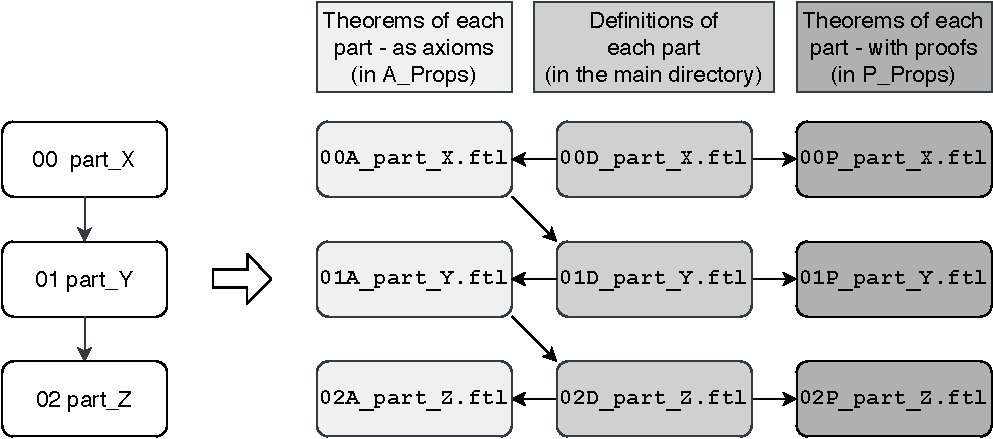
\includegraphics[scale=0.75]{./project_structure_explained.pdf}
}
\end{center}
\end{figure}

\subsection{The Implementation}

\subsubsection{The structure object}
Many of the objects we examine in this library have a similar structure. For examples groups, fields, vector spaces and rings all have a carrier, a zero element, and an addition defined on them. We introduce the object structure in 002D\_ structure.ftl. 
A structure is a function S such that the domain of S is a subset of language =  \{carrier, zero, one, addition, multiplication, negation, inverse, scalar multiplication\}. We can now define a each of the linear algebra structures above as a structure with then necessary components of language in its domain. 



\section{Comparison to Lean}


\section{Next Steps in Naproche}

Considering, that the naproche system is still in somewhat of a beta-phase we propose the following ideas to better the programming experience.
Firstly naproche needs an increase transparency in what the e-prover is doing. On the one hand the e-prover is a huge blessing, simplifying many steps. On the other hand it is the source of many problems, since the programmer can not guess where the e-prover is gets stuck. Also the e-prover will often take longer or even cant compile working code, if it is copied to a later part of the file. This is due to the increased breadth of the internal search tree. To counter these effects, while keeping the luxury of an assisting e-prover, we suggest the e-prover return the proofs of each statement, which can then be either pasted into the code or be saved in a separate file. This decoupling of the e-prover to the checking process will not only save time, but also guarantee more stability. 




\end{document}

